As with the reduction, individual scans can be combined into larger scans. Doing this, small individual scans can run in individual thread blocks, thereby enabling the usage of shared memory. The visual representation in \cref{fig:scan_blocking} shows a 1D implementation strategy for scanning of arrays larger than maximum block thread sizes.

\begin{figure}[ht]
	\centering
	\fbox{
		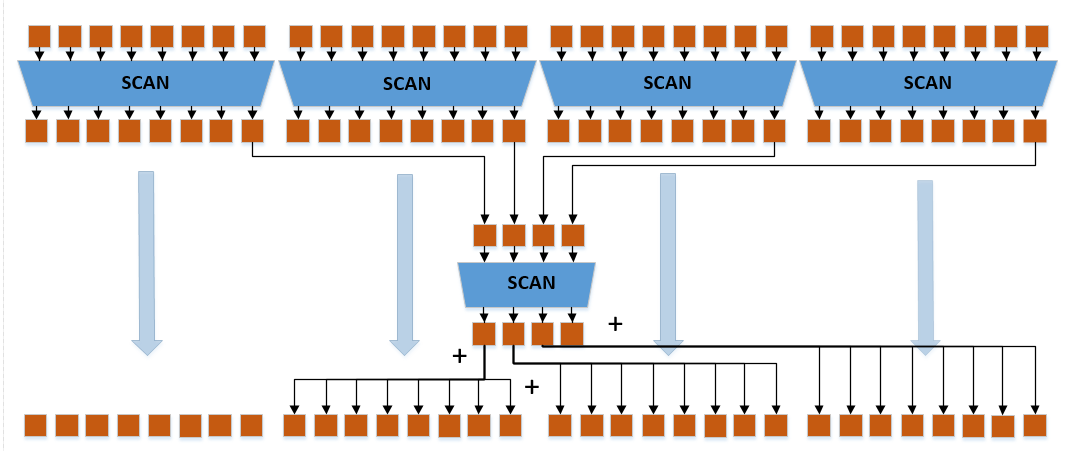
\includegraphics[width=0.9\textwidth]{figs/algorithm/scan_blocking.png}}
	\caption{Scanning of arbitrary array sizes, where individual thread block, run independent scan, later combined to the final array}
	\label{fig:scan_blocking}
\end{figure}

The idea is to divide the array into smaller arrays each with a maximum array size of the maximum threads per block. Then a individual scan is perform on each of the individual arrays. The reduction sum of each array is collected into a new array, on which a scan is performed, creating all the partial sums of the input array. The partial sums are summed with there respective individual array, thereby creating the total scanned output. 